\documentclass[PI,LAB]{HSEUniversity}

\usepackage{graphicx}
\graphicspath{ {img/} }

\usepackage{hyperref}
\hypersetup{
    colorlinks=true,
    linkcolor=black,
    filecolor=magenta,      
    urlcolor=cyan,
}

\title{Организация паттернов проектирования. Структурный паттерн <<Компоновщик>>}
\author{Рязанов Иван Дмитриевич}
\supervisor{к.т.н., доцент кафедры Информационных технологий в бизнесе НИУ ВШЭ-Пермь}{А.В.~Кычкин}
\Year{2020}

\begin{document}
\maketitle
\chapter{Паттерн <<Компоновщик>>}
\textbf{Название и классификация паттерна.}
Компоновщик - паттерн, структурирующий объекты.

\textbf{Назначение.}
Компонует объекты в древовидные структуры для представления иерархий часть-целое. Позволяет клиентам единообразно трактовать индивидуальные и составные объекты.
Управление группами объектов может быть непростой задачей, особенно, если эти объекты содержат собственные объекты. Паттерн компоновщик описывает, как можно применить рекурсивную композицию таким образом, что клиенту не придется проводить различие между простыми и составными объектами.

\textbf{Применимость.}
Использование паттерна Компоновщик целесообразно если:
\begin{enumerate}
  \item Необходимо объединять группы схожих объектов и управлять ими. 
  \item Объекты могут быть как примитивными (элементарными), так и составными (сложными). Составной объект может включать в себя коллекции других объектов, образуя сложные древовидные структуры. Пример: директория файловой системы состоит из элементов, каждый их которых также может быть директорией. 
  \item Код клиента работает с примитивными и составными объектами единообразно.
\end{enumerate}
\clearpage

\begin{figure}[p]
  \centering
  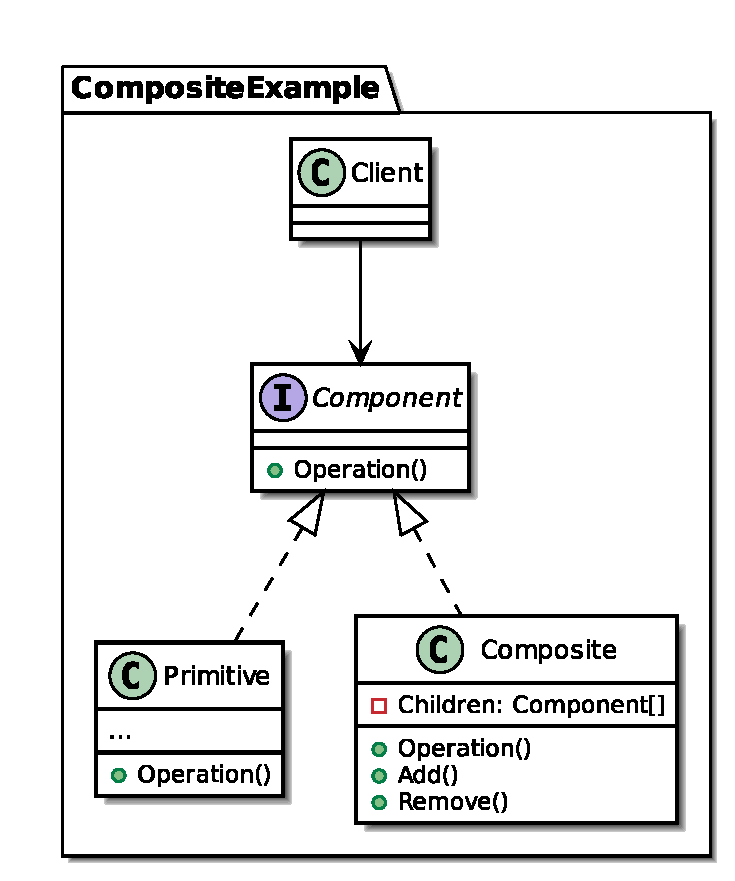
\includegraphics[scale=0.7]{Composite_CD.eps}
  \caption{Диаграмма классов паттерна <<Компоновщик>>}
\end{figure}

\begin{figure}[p]
  \centering
  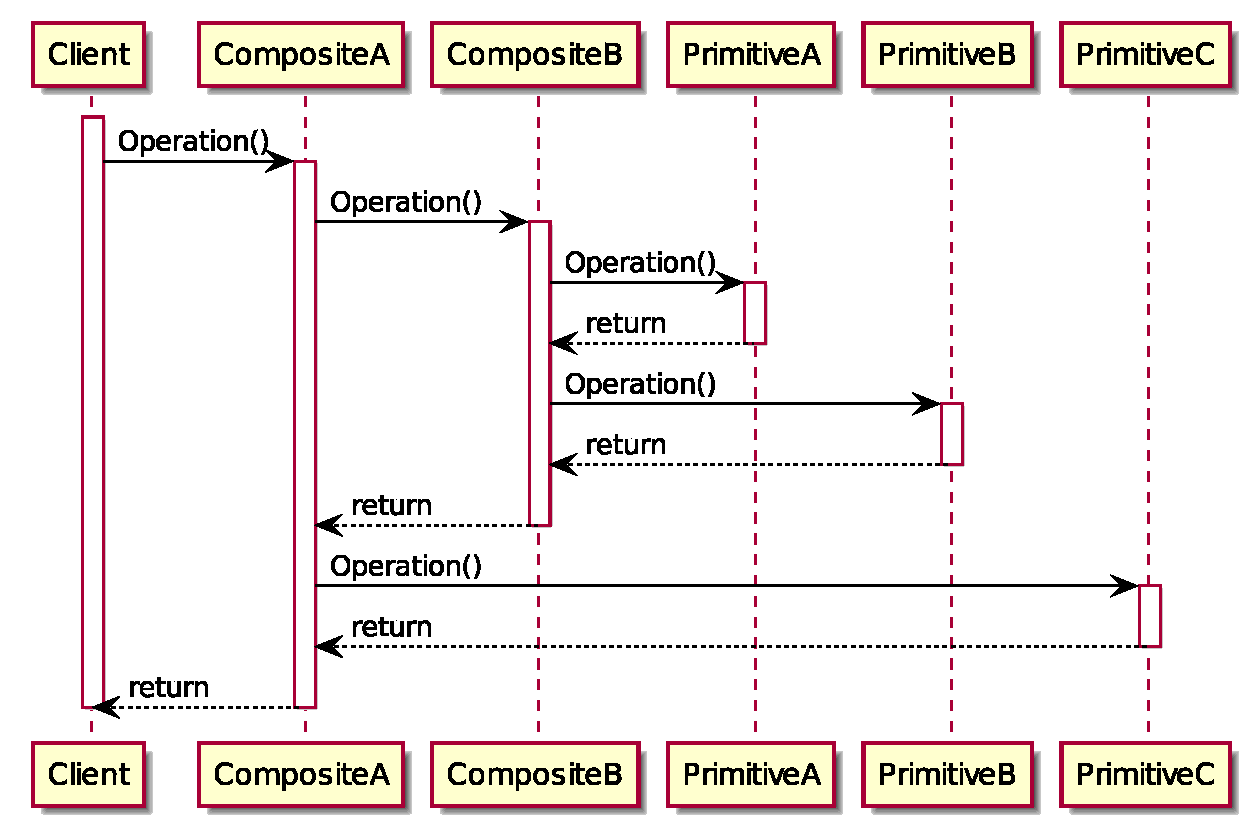
\includegraphics[scale=0.75]{Composite_SD.eps}
  \caption{Диаграмма последовательности паттерна <<Компоновщик>>}
\end{figure}
\clearpage

\textbf{Участники}

\begin{enumerate}
  \item Component --- компонент: - объявляет интерфейс для компонуемых объектов; предоставляет подходящую реализацию операций по умолчанию, общую для всех классов; объявляет интерфейс для доступа к потомкам и управления ими; определяет интерфейс для доступа к родителю компонента в рекурсивной структуре и при необходимости реализует его. Описанная возможность необязательна;
  \item Primitive (PrimitiveA, PrimitiveB, PrimitiveC) --- примитив: - представляет листовые узлы композиции и не имеет потомков; определяет поведение примитивных объектов в композиции;
  \item Composite (CompositeA, CompositeB) --- составной объект: определяет поведение компонентов, у которых есть потомки; хранит компоненты-потомки; реализует относящиеся к управлению потомками операции в интерфейсе класса Component;
  \item Client --- клиент: - манипулирует объектами композиции через интерфейс Component.
\end{enumerate}

\textbf{Отношения}

Клиенты используют интерфейс класса Component для взаимодействия с объектами в составной структуре. Если получателем запроса является дочерний объект Primitive, то он и обрабатывает запрос. Когда же получателем является составной объект Composite, то обычно он перенаправляет запрос своим потомкам, возможно, выполняя некоторые дополнительные операции до или после перенаправления.

\textbf{Плюсы и минусы}

Плюсы:
\begin{enumerate}
  \item В систему легко добавлять новые примитивные или составные объекты, так как паттерн Composite использует общий базовый класс Component;
  \item Код клиента имеет простую структуру – примитивные и составные объекты обрабатываются одинаковым образом;
  \item Паттерн Composite позволяет легко обойти все узлы древовидной структуры.
\end{enumerate}

Минусы:
\begin{enumerate}
  \item Неудобно осуществить запрет на добавление в составной объект Composite объектов определенных типов. Так, например, в состав Умного дома не могут входить станки с числовых программным управлением (ЧПУ).
\end{enumerate}

\textbf{Области применения}

\begin{enumerate}
  \item Приложение, которое требует базовой функциональности во всей своей иерархической структуре.
  \item GUI приложений. 
\end{enumerate}

\chapter{Проектирование и реализация}
\section{Проектирование}
Для реализации был выбран 2 вариант:

<<Описание сценариев Умного дома. Описание различных функций, получаемых путем комбинации датчиков, исполнительных механизмов, панелей оператора, мультимедиа систем, контроллеров управления, сетевых устройств.>>

Перед началом работы построим диаграмму классов (см. рис. \ref{fig:Task_CD}).
 \begin{figure}[p]
   \centering
   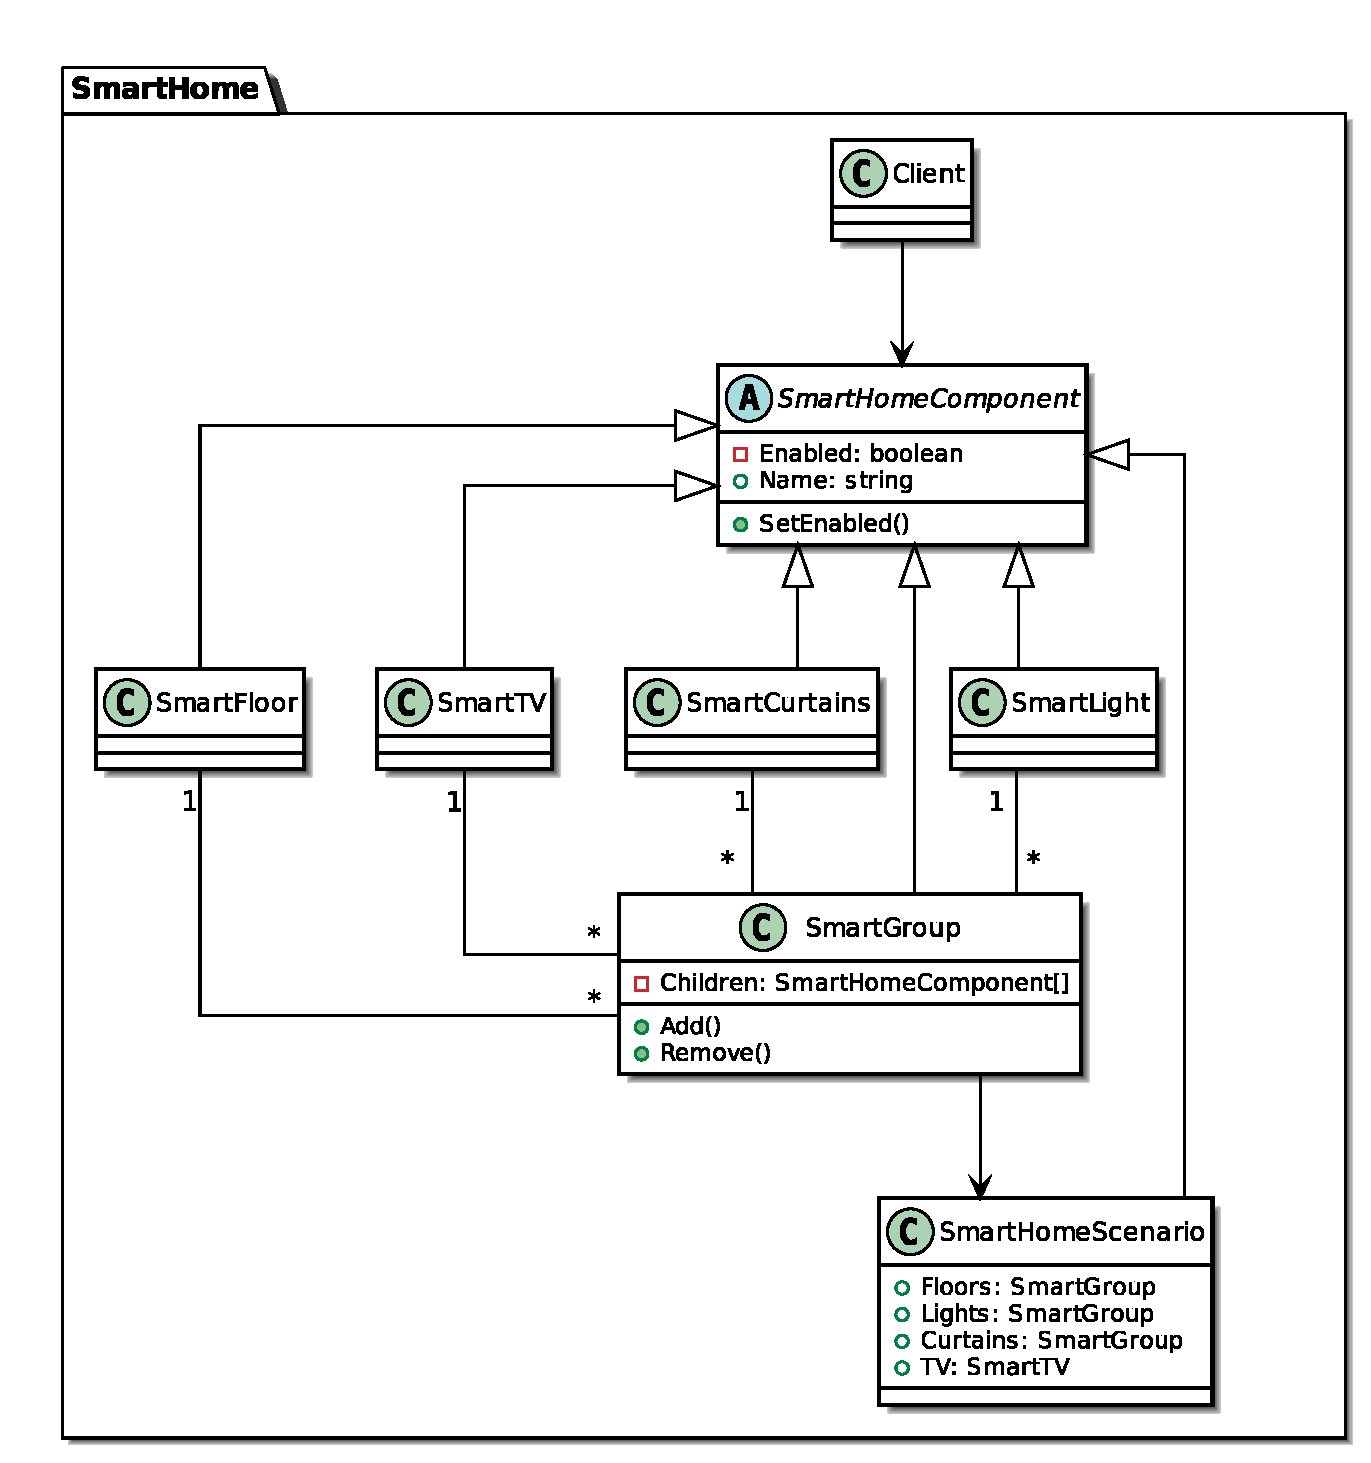
\includegraphics[scale=0.75]{Task_CD.eps}
   \caption{Диаграмма классов}
   \label{fig:Task_CD}
 \end{figure}

\textbf{Участники}

\begin{enumerate}
  \item SmartHomeComponent --- компонент умного дома: - содержит поле с названием компонета и статус (активен или неактивен). Имеет метод для активации/деактивации. 
  \item SmartTV, SmartLight, SmartCurtains, SmartFloor --- примитивы, компоненты умного дома. 
  \item SmartHomeScenario --- сценарий умного дома - содержит массив элементов, которыми сценарий управляет.
  \item Client --- клиент: - запускает сценарии умного дома через объекты SmartHomeScenario.
\end{enumerate}

\section{Реализация}
Реализация паттерна <<Компоновщик>> находится в git-репозитории по ссылке: \href{https://github.com/rovany706/design-patterns/}{github.com}

\end{document}
